\documentclass[11pt,letterpaper]{article}
% PDF reproductible : sans date de compilation ni identifiant aleatoire, pour que git ne voie pas
% de changement quand le contenu est le meme
\pdfinfoomitdate=1
\pdftrailerid{}
\pdfsuppressptexinfo=-1
%graph pour image H
\usepackage{float}

% Pour Dessin
\usepackage{tikz}
\usepackage{amsmath}
\usetikzlibrary{arrows.meta, positioning, patterns, decorations.pathreplacing}

% packetages pour ecrire en français
\usepackage[french]{babel}
\usepackage[utf8]{inputenc}
\usepackage[T1]{fontenc}

% pour les maths, les graphiques et la navigation dans le pdf
\usepackage{amsmath, amssymb, mathtools, bm, array}
\usepackage{graphicx,caption,subcaption}
\graphicspath{{./}}
\usepackage{hyperref}
\hypersetup{
    pdftitle={Sismique réfraction sous le Grand Axe de l'Université Laval},
    pdfauthor={L-F. Brodeur (LFBRO1), S. L-Tremblay (SILAT10)}
}

% marges, police de caractère et header
\usepackage{geometry}
\geometry{top=23mm, bottom=23mm, left=20mm, right=20mm}
\usepackage{cochineal}
\usepackage{fancyhdr}
\pagestyle{fancy}

\parindent=0mm % pas d'indentation

\lhead{L-F. Brodeur (IDUL: LFBRO1) et S. L-Tremblay (IDUL: SILAT10)}
\rhead{Géophysique: sismique réfraction}
\fancyheadoffset{0 cm}

\setlength{\headheight}{13.6pt}

% Bibliographie: une reference n'apparait que si elle est citee dans le texte.
% \cite ecrit \citation{cle} dans le .aux, relu au debut du document a la compilation suivante.
\makeatletter
\def\citation#1{\@for\@clecitee:=#1\do{\expandafter\gdef\csname refcitee@\@clecitee\endcsname{}}}
\newcommand{\refsicitee}[2]{\@ifundefined{refcitee@#1}{}{\bibitem{#1}#2}}
\makeatother

% commandes pour ecrire des equations plus vite avec leur label
\newcommand{\beq}[1]{\begin{equation} \label{#1}}
\def\enq{\end{equation}}

% C'est parti!
\begin{document}
\shorthandoff{;:!?}
\thispagestyle{empty} % pas de header sur la première page
\begin{center}

\noindent
\begin{minipage}[t]{0.5\textwidth}
\raggedright
{\large GPH-3000 \textit{Travaux pratiques avancés}}\\
{\large Automne 2026 $\vert$ GPH-3000 (Groupe: 85213)}
\end{minipage}%
\begin{minipage}[t]{0.5\textwidth}
\raggedleft
{\large \textsc{L-F. Brodeur (IDUL: LFBRO1)}}\\
{\large \textsc{S. L-Tremblay (IDUL: SILAT10)}}
\end{minipage}
\\~\\
\vspace{1em}
{\Large \textbf{Sismique réfraction sous le Grand Axe de l'Université Laval} }\\
[0.3em]
{\large Date du Laboratoire: 15 octobre 2026 \qquad\qquad\qquad Remis le \today}

\end{center}

\vspace{0.5em}
\subsection*{Résumé}
Sous le gazon du Grand Axe se trouve du roc qu'on ne voit pas normalement, mais dont on peut estimer la profondeur avec un coup de masse sur le sol. Lorsqu'on frappe le sol, une onde traverse la première couche plus molle du sol et atteint une deuxième couche plus solide et donc où elle peut se déplacer plus rapidement. L'onde dans ce deuxième niveau plus rapide peut donc remonter à la surface et se rendre à un point plus rapidement que l'onde qui serait passée simplement dans la première couche molle. Dans cette expérience, trois géophones connectés sur un oscilloscope ont servi à enregistrer les ondes produites en frappant une plaque de métal à différentes distances entre 0,13 et 5,33~m. Le temps entre la frappe et la première onde détectée par un géophone est ensuite tracé en fonction de la distance. Ce graphique montre deux droites, la première pente donne une vitesse de $341 \pm 19~\text{m/s}$ dans la couche de surface et la deuxième une vitesse de $660 \pm 39~\text{m/s}$ dans la couche en dessous, et les deux droites se croisent à $1{,}44 \pm 0{,}22~\text{m}$. L'épaisseur de la couche de surface est donc de $0{,}41 \pm 0{,}07~\text{m}$. Par contre, une vitesse de 660~m/s semble trop basse pour du roc. En 1909, Andrija Mohorovičić a utilisé la même idée avec un tremblement de terre en Croatie: les ondes qui arrivaient plus tôt que prévu aux stations sismiques éloignées lui ont permis de découvrir la limite entre la croûte et le manteau, à environ 54~km de profondeur \cite{herak}.

\section{Introduction}

Sous la pelouse du campus de l'Université Laval, le roc est recouvert d'une couche de sol mou. Pour connaître l'épaisseur de ce sol sans creuser, on peut utiliser la sismique réfraction. Cette méthode mesure le temps avant qu'une onde soit détectée en fonction de la distance à laquelle cette onde a été générée à la surface. Les compagnies minières et pétrolières utilisent cette méthode pour mesurer le sous-sol depuis plus d'un siècle \cite{telford}.

L'objectif de l'expérience était de mesurer la profondeur du roc sous le Grand Axe par sismique réfraction. La Section~\ref{sec:theorie} présente les calculs théoriques pour utiliser les temps d'arrivée de l'onde directe et de l'onde réfractée pour mesurer l'épaisseur de la couche de la surface. La Section~\ref{sec:methodologie} décrit l'endroit où l'expérience a été réalisée, la méthode d'acquisition et le traitement des données. Les résultats sont présentés à la Section~\ref{sec:resultats}. La Section~\ref{sec:discussion} discute des caractéristiques des couches mesurées. La Section~\ref{sec:conclusion} conclut.

\section{Théorie}
\label{sec:theorie}

On considère une couche de surface d'épaisseur $e$ où les ondes voyagent à la vitesse $V_1$. Cette couche est sur un milieu plus rapide de vitesse $V_2 > V_1$ (Figure~\ref{fig:schema}). Trois géophones à une distance $x$ de l'impact et espacés de 10~cm reçoivent l'onde directe qui arrive au temps
\beq{eq:directe}
    t_d = \frac{x}{V_1} .
\enq
Ils reçoivent aussi l'onde qui frappe l'interface à l'angle critique $\theta_c$, défini par $\sin\theta_c = V_1/V_2$ (loi de Snell). Cette onde voyage le long de l'interface à la vitesse $V_2$ et remonte vers la surface avec le même angle. Son temps d'arrivée est \cite{telford}
\beq{eq:refractee}
    t_r = \frac{x}{V_2} + \frac{2e\cos\theta_c}{V_1} = \frac{x}{V_2} + 2e\sqrt{\frac{1}{V_1^2} - \frac{1}{V_2^2}} .
\enq
Les deux temps augmentent linéairement avec $x$, mais l'onde réfractée a une pente plus petite. Proche de l'impact, l'onde directe arrive en premier mais, plus loin que la distance critique $D_c$ où $t_d = t_r$, c'est l'onde réfractée qui arrive en premier. Le graphique du temps de première arrivée en fonction de la distance donne donc deux droites, de pentes $1/V_1$ et $1/V_2$, qui se croisent à $D_c$. Avec $t_d = t_r$ à $x = D_c$, on peut calculer l'épaisseur de la couche de surface \cite{protocole}:
\beq{eq:epaisseur}
    e = \frac{D_c}{2}\sqrt{\frac{V_2 - V_1}{V_2 + V_1}} .
\enq

\section{Méthodologie}
\label{sec:methodologie}

\subsubsection*{Site et montage}
Les mesures ont été faites sur le Grand Axe de l'Université Laval, à côté du pavillon Adrien-Pouliot et du pavillon Alexandre-Vachon (Figure~\ref{fig:localisation}), en suivant le protocole du cours \cite{protocole}. Trois géophones verticaux ont été plantés dans le sol en ligne, séparés par 10~cm. Les ondes étaient générées en frappant avec une masse une plaque en métal sur le sol, à une distance dans l'axe de la ligne des 3 géophones. Le centre de la plaque, où frappe la masse, est à 13~cm de son bord. La plaque a été placée à dix distances $d$ du géophone 1 (G1), de 0 à 5~m. La distance entre l'impact et les géophones 1, 2 et 3 est donc $x = d + 0{,}13~\text{m}$, $d + 0{,}23~\text{m}$ et $d + 0{,}33~\text{m}$ (Figure~\ref{fig:schema}).

\begin{figure}[htbp]
    \centering
    \begin{subfigure}[b]{0.42\textwidth}
        \centering
        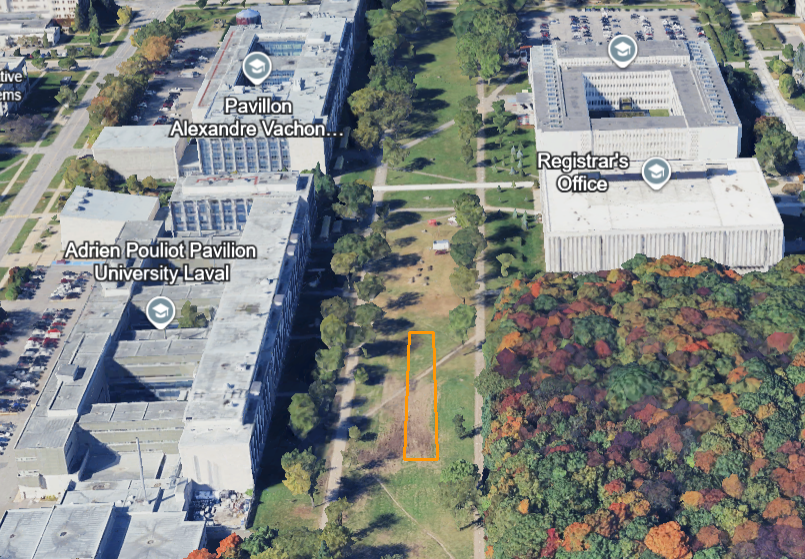
\includegraphics[width=\textwidth]{../figures/Localisation.png}
        \caption{}
        \label{fig:localisation}
    \end{subfigure}
    \hfill
    \begin{subfigure}[b]{0.54\textwidth}
        \centering
        \begin{tikzpicture}[scale=1.0, >=Stealth]
            % couches
            \fill[brown!20] (-0.6,0) rectangle (8.0,-1.6);
            \fill[brown!45] (-0.6,-1.6) rectangle (8.0,-3.0);
            \draw[thick] (-0.6,0) -- (8.0,0);
            \draw (-0.6,-1.6) -- (8.0,-1.6);
            \node[left] at (8.0,-0.3) {$V_1$};
            \node[left] at (8.0,-2.7) {$V_2$};
            % epaisseur
            \draw[<->] (-0.3,0) -- (-0.3,-1.6) node[midway, right] {$e$};
            % plaque et masse
            \fill[gray!70] (0.0,0) rectangle (2.4,0.15);
            \draw[->, very thick] (1.2,1.8) -- (1.2,0.22);
            \node[above] at (1.2,1.8) {masse};
            % geophones
            \foreach \x/\n in {4.0/1, 5.0/2, 6.0/3} {
                \fill (\x-0.13,0) -- (\x+0.13,0) -- (\x,0.3) -- cycle;
                \node[above] at (\x,0.32) {\small G\n};
            }
            % cotes: lignes de rappel, puis fleches aux deux bouts a la meme hauteur
            \draw[gray] (2.4,0.2) -- (2.4,1.2);
            \foreach \x in {4.0, 5.0} {\draw[gray] (\x,0.75) -- (\x,1.2);}
            \draw[<->] (1.2,1.05) -- (2.4,1.05) node[midway, above] {\small 13~cm};
            \draw[<->] (2.4,1.05) -- (4.0,1.05) node[midway, above] {$d$};
            \draw[<->] (4.0,1.05) -- (5.0,1.05) node[midway, above] {\small 10~cm};
            % trajets
            \draw[dashed, red!70!black, thick, ->] (1.2,0) -- (2.4,-1.6) -- (4.8,-1.6) -- (6.0,0);
            \draw[blue!70!black, thick, ->] (1.2,-0.25) -- (5.9,-0.25);
            \node[blue!70!black, below] at (3.6,-0.25) {\small onde directe};
            \node[red!70!black, below] at (3.6,-1.6) {\small onde réfractée};
            % angle critique a l'entree et a la sortie (etiquette sur la bissectrice)
            \draw (2.4,-1.6) -- (2.4,-0.8);
            \draw (2.4,-1.1) arc (90:126.87:0.5);
            \node at ({2.4+1.0*cos(108.43)},{-1.6+1.0*sin(108.43)}) {\small $\theta_c$};
            \draw (4.8,-1.6) -- (4.8,-0.8);
            \draw (4.8,-1.1) arc (90:53.13:0.5);
            \node at ({4.8+1.0*cos(71.57)},{-1.6+1.0*sin(71.57)}) {\small $\theta_c$};
        \end{tikzpicture}
        \caption{}
        \label{fig:schema}
    \end{subfigure}
    \caption{(a) Site où ont été faites les mesures (rectangle orange), image tirée de Google Earth. (b) Schéma de la plaque, des trois géophones et du trajet de l'onde directe et de l'onde réfractée (pas à l'échelle).}
    \label{fig:site}
\end{figure}

\subsubsection*{Acquisition}
Les 3 géophones étaient branchés sur 3 canaux d'un oscilloscope à quatre canaux. Le quatrième canal recevait un signal de 9~V qui tombait à 0~V lorsque la masse entrait en contact avec la plaque et fermait un circuit. L'oscilloscope était déclenché sur le front descendant de ce quatrième canal et était utilisé pour obtenir le $t = 0$. L'échelle de chaque canal était ajustée à l'amplitude des signaux à chaque distance. Trois coups ont été enregistrés à chaque distance, ce qui donne un total de 30 enregistrements.

\subsubsection*{Repérage des premières arrivées}
L'analyse a été faite en Python. Pour chaque distance et chaque géophone, les trois enregistrements sont divisés par l'écart-type de leur bruit avant l'impact et sont additionnés et filtrés sur 0,5~ms pour réduire le bruit. Le temps d'arrivée est défini comme le premier moment où le signal passe par dessus $\pm 2$ fois le niveau du bruit et y reste pendant 0,5~ms.

Après, les temps d'arrivée en fonction de la distance sont ajustés avec un curve fit de deux droites qui se croisent à $D_c$ (Figure~\ref{fig:dromo}). L'équation du modèle pour le curve fit est
\beq{eq:modele}
    t(x) =
    \begin{cases}
        x/V_1 & x < D_c \\
        D_c/V_1 + (x - D_c)/V_2 & x \geq D_c
    \end{cases} .
\enq
La première droite part de l'origine parce que l'impact à $x = 0$ est nécessairement détecté à $t = 0$ (équation~\ref{eq:directe}). L'épaisseur $e$ peut être calculée avec l'équation~\ref{eq:epaisseur}. Son incertitude est propagée par dérivées partielles à partir des incertitudes sur $D_c$, $V_1$ et $V_2$ données par la matrice de covariance de l'ajustement:
\beq{eq:incertitude}
    \Delta e = e\sqrt{\left(\frac{\Delta D_c}{D_c}\right)^2 + \left(\frac{V_2\,\Delta V_1}{V_2^2 - V_1^2}\right)^2 + \left(\frac{V_1\,\Delta V_2}{V_2^2 - V_1^2}\right)^2} .
\enq

\section{Résultats}
\label{sec:resultats}

La Figure~\ref{fig:section} montre les signaux moyens du géophone 3 pour les dix distances. On y voit aussi le point que la règle a déterminé comme étant l'arrivée de la première onde et l'ajustement du curve fit.

\begin{figure}[htbp]
    \centering
    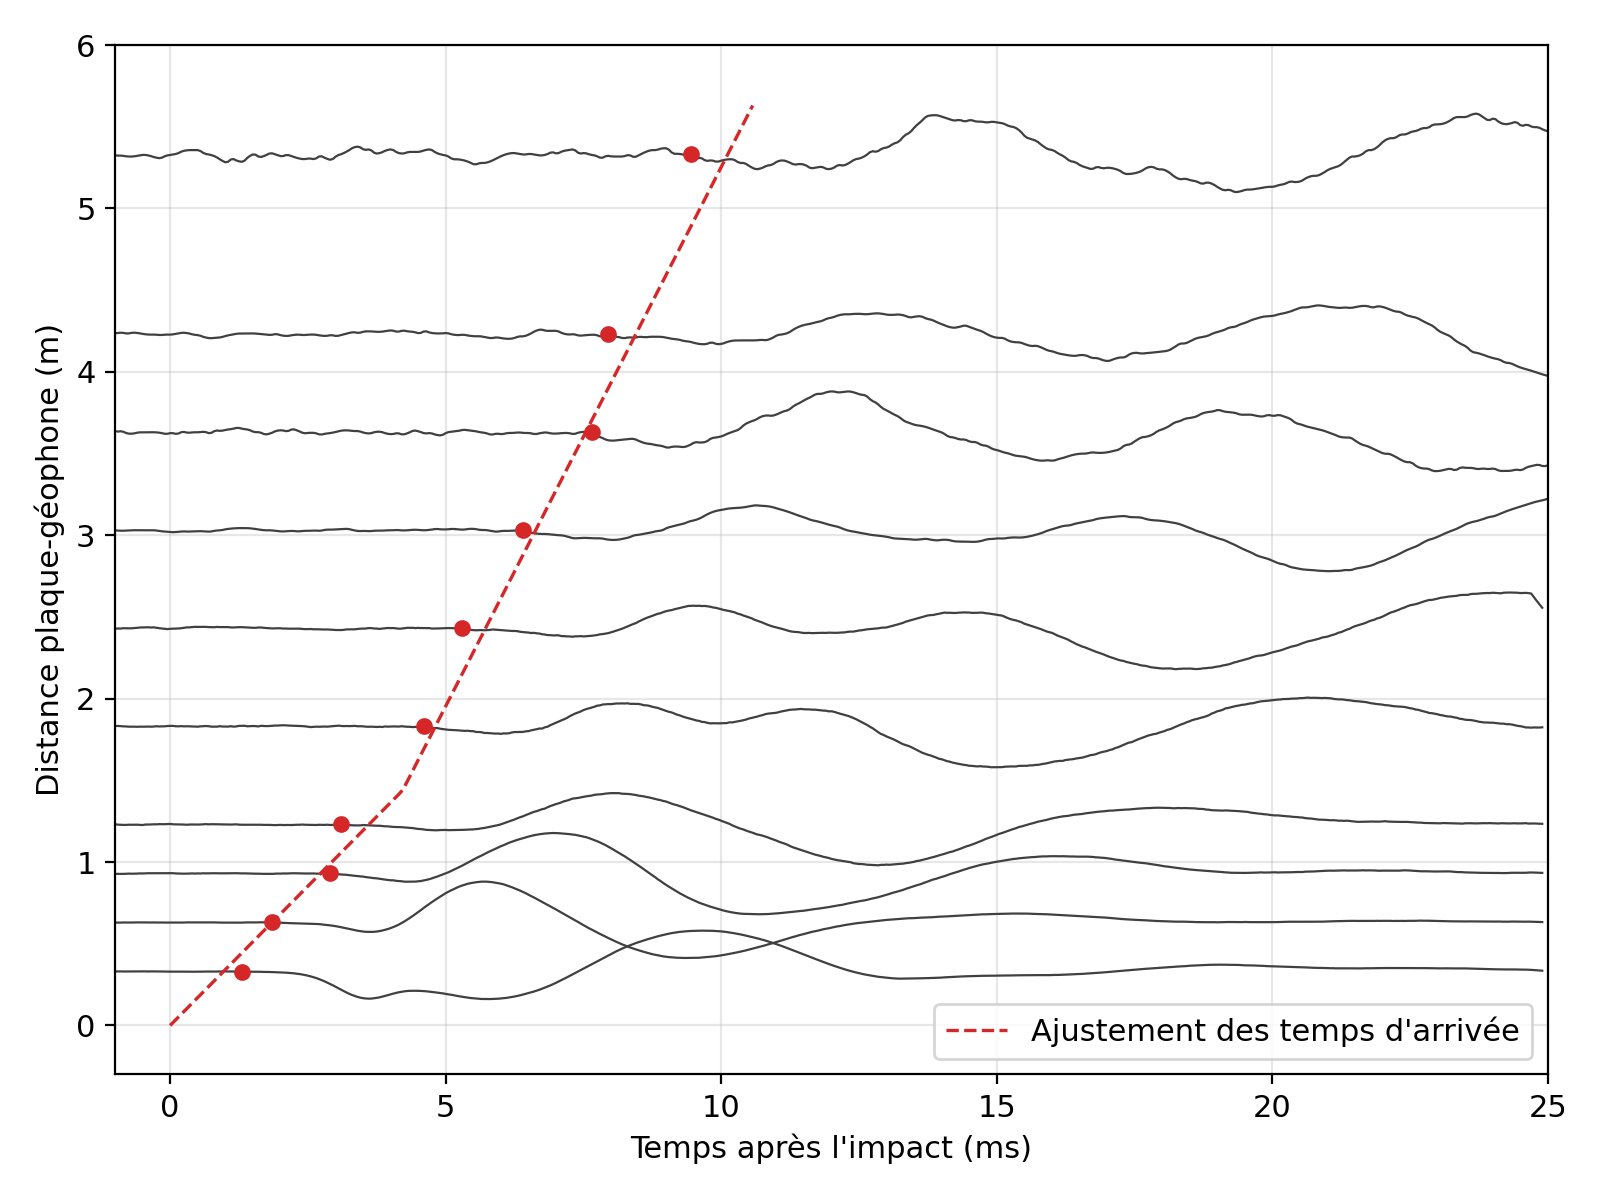
\includegraphics[width=0.74\textwidth]{../figures/01_section_sismique.png}
    \caption{Signal moyen des trois coups de masse au géophone 3 pour chaque distance. Les points rouges montrent les temps de la première arrivée et la ligne pointillée l'ajustement du curve fit (équation~\ref{eq:modele}).}
    \label{fig:section}
\end{figure}

Le Tableau~\ref{tab:temps} donne les temps de la première arrivée pour chaque distance pour les 3 géophones. Le signal du géophone 2 à 3,9~m a été rejeté, parce que la première arrivée est invisible dans le bruit.

\begin{table}[htbp]
\centering
\caption{Temps de première arrivée aux trois géophones pour chaque position de la plaque. Le tiret indique une première arrivée noyée dans le bruit.}
\label{tab:temps}
\small
\begin{tabular}{cccc}
\hline
$d$ (m) & $t$, géophone 1 (ms) & $t$, géophone 2 (ms) & $t$, géophone 3 (ms) \\
\hline
0,0 & 1,65 & 1,40 & 1,30 \\
0,3 & 1,30 & 1,10 & 1,85 \\
0,6 & 2,45 & 2,50 & 2,90 \\
0,9 & 2,95 & 3,35 & 3,10 \\
1,5 & 4,35 & 4,80 & 4,60 \\
2,1 & 5,50 & 6,10 & 5,30 \\
2,7 & 6,20 & 6,95 & 6,40 \\
3,3 & 7,40 & 7,30 & 7,65 \\
3,9 & 8,20 & --- & 7,95 \\
5,0 & 9,95 & 10,70 & 9,45 \\
\hline
\end{tabular}
\\[0.3em]
\end{table}

Ces temps sont tracés en fonction de $x$ à la Figure~\ref{fig:dromo}. L'ajustement de l'équation~\ref{eq:modele} donne
\begin{equation*}
    V_1 = 341 \pm 19~\text{m/s}, \qquad V_2 = 660 \pm 39~\text{m/s}, \qquad D_c = 1{,}44 \pm 0{,}22~\text{m},
\end{equation*}
avec $R^2 = 0{,}978$. Les vitesses viennent des pentes $s = 1/V$, donc $\Delta V = \Delta s/s^2$. L'écart quadratique moyen des points autour de l'ajustement est de 0,42~ms. Cette valeur est utilisée comme incertitude sur chaque temps d'arrivée (barres d'erreur de la Figure~\ref{fig:dromo}). Avec les équations~\ref{eq:epaisseur} et~\ref{eq:incertitude}, l'épaisseur de la couche de surface est
\beq{eq:resultat}
    e = 0{,}41 \pm 0{,}07~\text{m} .
\enq

\begin{figure}[htbp]
    \centering
    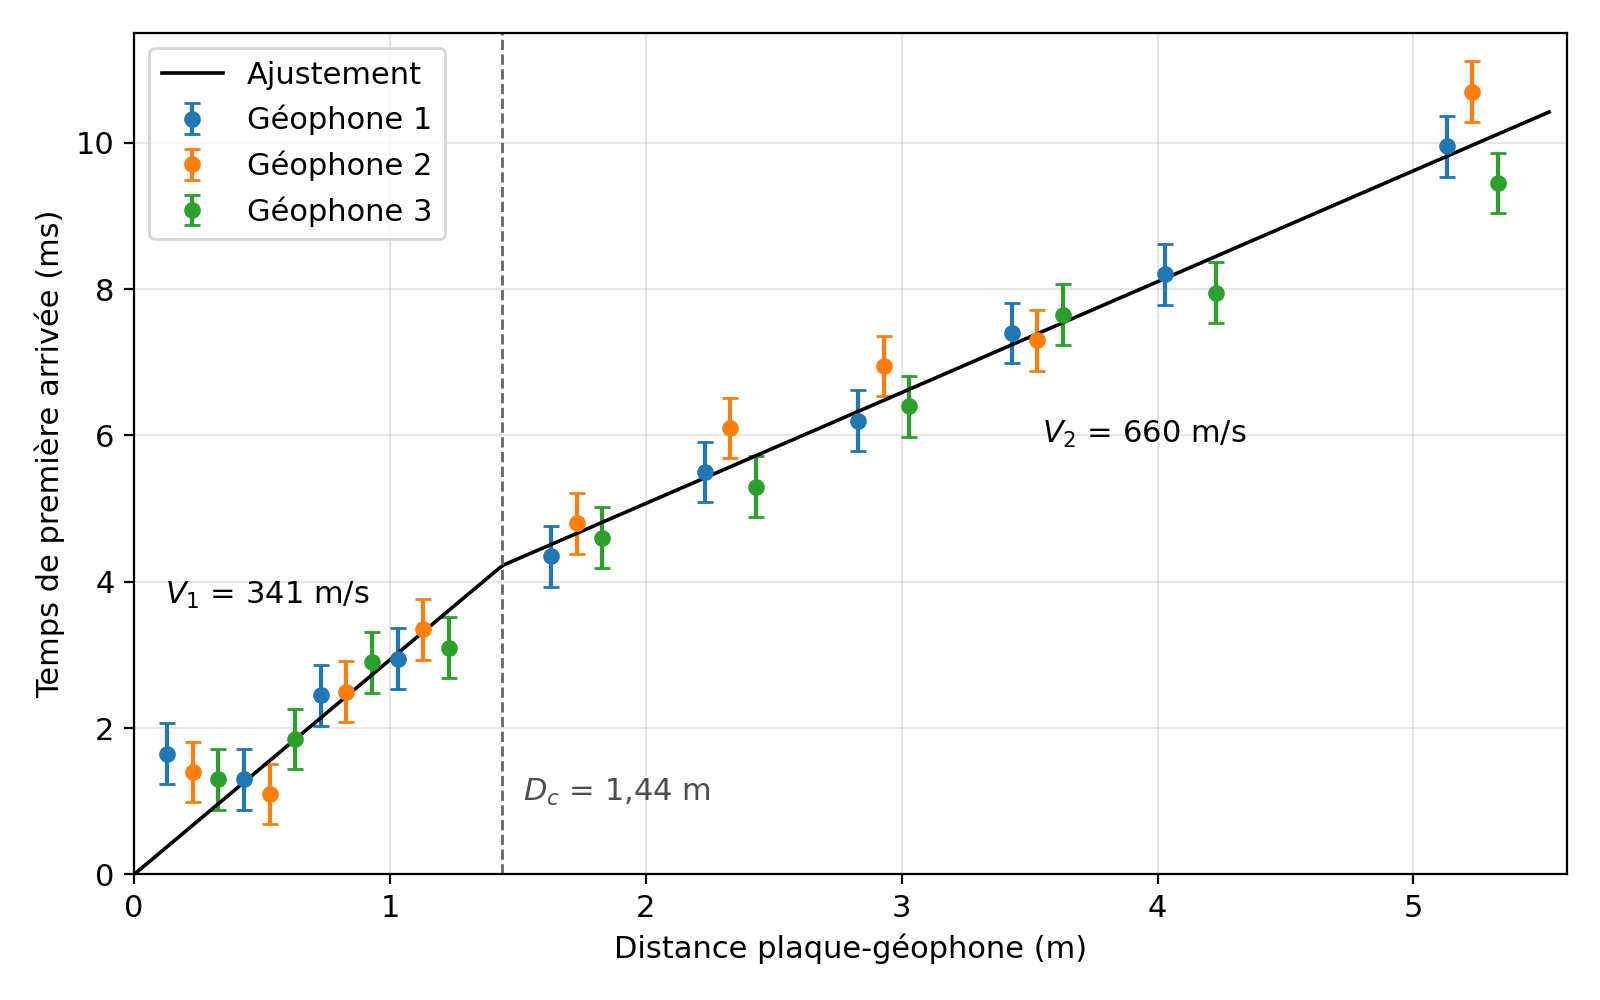
\includegraphics[width=0.78\textwidth]{../figures/02_dromochronique.png}
    \caption{Temps de première arrivée en fonction de la distance entre l'impact et le géophone. La ligne pointillée grise marque la distance critique $D_c$ où les deux droites se croisent.}
    \label{fig:dromo}
\end{figure}

\section{Discussion}
\label{sec:discussion}

\subsubsection*{Nature des deux couches}
Les deux vitesses mesurées sont typiques de sols mous. Les ondes de pression voyagent entre 200 et 1000~m/s dans un sable sec et à plus de 1500~m/s dans un sol saturé en eau \cite{reynolds}. La couche de surface ($V_1 = 341~\text{m/s}$) correspond donc probablement à la terre végétale. La couche en dessous ($V_2 = 660~\text{m/s}$) est plus compacte, mais sa vitesse est trop petite pour du roc. L'interface mesurée à 0,41~m n'est donc probablement pas le roc, mais une limite entre deux couches de sol mou.

\subsubsection*{Incertitude sur l'épaisseur}
L'incertitude relative de 16~\% sur $e$ vient presque entièrement de $D_c$ (15~\%). Le coude entre les deux droites tombe entre les mesures à $x = 1{,}23$ et $1{,}63~\text{m}$, où il n'y a aucun point, et sa position est donc difficile à déterminer avec précision. Les autres sources d'incertitude sont petites comparées à l'écart quadratique moyen de 0,42~ms sur les temps.

Le modèle nous oblige à ce que la première droite parte de l'origine. Par contre, les trois points les plus proches de la plaque ($x \leq 0{,}33~\text{m}$) sont tous au-dessus de cette droite, de 0,3 à 1,3~ms (Figure~\ref{fig:dromo}). Cela pointe vers une erreur provenant de la largeur de la plaque car l'onde n'est pas émise par une singularité mais bien par une plaque de 26~cm de longueur sur la ligne des géophones.

Le modèle suppose aussi des couches parfaitement horizontales, uniformes et avec des interfaces propres. Ces conditions ne sont probablement pas respectées dans la réalité, ce qui peut aider à expliquer l'écart quadratique moyen de 0,42~ms.

\section{Conclusion}
\label{sec:conclusion}

Trois géophones et un oscilloscope déclenché par une masse ont permis de mesurer les temps de première arrivée des ondes sismiques. Ces temps montrent deux couches du sol: une couche de surface de $0{,}41 \pm 0{,}07~\text{m}$ où les ondes de pression voyagent à 341~m/s et une couche plus rapide à 660~m/s. Cette deuxième vitesse est trop petite pour du roc. L'objectif de mesurer la profondeur du roc n'a donc pas été atteint, mais on peut dire qu'il se trouve à plus de 2,2~m. Une plus grande sensibilité avec des coups de masse plus éloignés pourrait servir à déterminer la réelle épaisseur du roc.

\renewcommand{\refname}{Bibliographie}
\begin{thebibliography}{9}

\refsicitee{protocole}{%
Département de physique, de génie physique et d'optique, Université Laval. \textit{GPH-3000, Travaux pratiques avancés: Géophysique (Sismique-réfraction)}, version 2019-09-23, et \textit{Expérience de sismique-réfraction: résumé des manipulations}, version 2022-09-22.}

\refsicitee{telford}{%
Telford, W.M., Geldart, L.P. et Sheriff, R.E. \textit{Applied Geophysics}, 2\textsuperscript{e} édition. Cambridge University Press, 1990.}

\refsicitee{reynolds}{%
Reynolds, J.M. \textit{An Introduction to Applied and Environmental Geophysics}, 2\textsuperscript{e} édition. Wiley-Blackwell, 2011.}

\refsicitee{bape}{%
Ministère des Transports du Québec. \textit{Réaménagement de l'échangeur Jean-Lesage: étude d'impact sur l'environnement}, document PR3.1, partie 2. Bureau d'audiences publiques sur l'environnement. \url{https://archives.bape.gouv.qc.ca/sections/mandats/echangeur_jean-lesage/documents/PR3.1,\%20partie2de4.pdf} (consulté en octobre 2026).}

\refsicitee{herak}{%
Herak, D. et Herak, M. « Andrija Mohorovičić (1857--1936): On the occasion of the 150th anniversary of his birth ». \textit{Seismological Research Letters}, vol. 78, n\textsuperscript{o} 6, p. 671--674, 2007.}

\end{thebibliography}

\end{document}
